\documentclass[tikz,border=5pt]{standalone}
\usepackage[UTF8]{ctex}
\usepackage{amsmath,amssymb}
\usetikzlibrary{arrows.meta,calc,angles,quotes,patterns,decorations.pathmorphing}
\definecolor{field}{HTML}{176B9B}
\definecolor{force}{HTML}{B64B32}
\tikzset{>=Latex,line width=.8pt,every node/.style={font=\small},field/.style={color=field},force/.style={color=force},body/.style={draw=black,fill=blue!6},ghost/.style={dashed,gray},labelbox/.style={fill=white,inner sep=1.5pt}}
\begin{document}
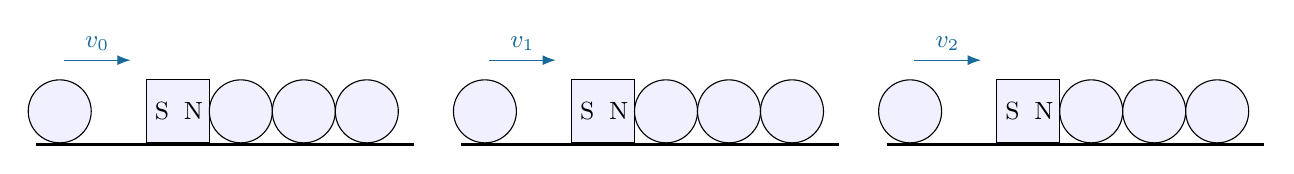
\begin{tikzpicture}
\foreach \k in{0,1,2}{
\begin{scope}[xshift=5.4*\k cm]
\draw[thick] (-1.8,-.42)--(3,-.42);
\draw[body] (-.4,-.4) rectangle(.4,.4);
\node at(-.2,0){S};\node at(.2,0){N};
\foreach\x in{.8,1.6,2.4}\draw[body](\x,0)circle(.4);
\draw[body](-1.5,0)circle(.4);
\draw[->,field](-1.45,.65)--(-.6,.65)node[midway,above]{$v_{\k}$};
\end{scope}}
\end{tikzpicture}
\begin{tikzpicture}
\draw[body] (-.45,-.45) rectangle(.45,.45);\node at(0,0){磁铁};
\foreach\x in{.9,1.8,2.7}\draw[body](\x,0)circle(.45);
\foreach\x in{0,.9,2.7}\fill(\x,0)circle(1pt);
\draw[<->] (0,-.9)--(.9,-.9)node[midway,below]{$2r$};
\draw[<->] (0,-1.5)--(2.7,-1.5)node[midway,below]{$6r$};
\draw[<->] (3.35,0)--(3.35,.45)node[midway,right]{$r$};
\draw[->,field] (2.7,.8)--(4,.8)node[right]{$w$};
\draw[->,force](-2,0)--(-.8,0)node[midway,above]{$K/x^3$};
\draw[ghost] (0,0)--(0,-1.5);\draw[ghost](2.7,0)--(2.7,-1.5);
\node[above] at(0,.65){固定阶段};
\end{tikzpicture}
\begin{tikzpicture}
\foreach \k in{0,1,2,3}{
\begin{scope}[yshift=-1.25*\k cm]
\foreach\j in{0,...,4}{
\ifnum\j=1
\draw[body](1.6*\j-.4,-.35)rectangle(1.6*\j+.4,.35);
\else\draw[body](1.6*\j,0)circle(.35);\fi
}
\draw[->,field,thick](1.6*\k,.55)--++(.9,0)node[right]{$a_e^{\k}u$};
\draw[->,force](1.6*\k+.42,0)--++(.6,0);
\node[left] at(-.5,0){第\the\numexpr\k+1\relax 次};
\end{scope}}
\node[below]at(0,-4.25){入射球};
\node[below]at(1.6,-4.25){磁铁};
\node[below]at(4.8,-4.25){三颗靶球};
\node[right]at(7.2,-2){$a_e=(1+e)/2$};
\end{tikzpicture}
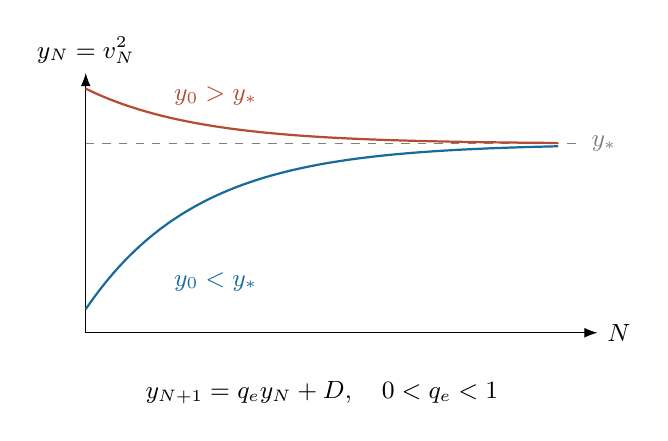
\begin{tikzpicture}
\draw[->](0,0)--(6.5,0)node[right]{$N$};
\draw[->](0,0)--(0,3.3)node[above]{$y_N=v_N^2$};
\draw[ghost](0,2.4)--(6.3,2.4)node[right]{$y_*$};
\draw[field,thick,domain=0:6,samples=70]plot(\x,{2.4-2.1*exp(-.7*\x)});
\draw[force,thick,domain=0:6,samples=70]plot(\x,{2.4+.7*exp(-.7*\x)});
\node[field,right]at(1,.65){$y_0<y_*$};
\node[force,right]at(1,3){$y_0>y_*$};
\node[below]at(3,-.5){$y_{N+1}=q_e y_N+D,\quad 0<q_e<1$};
\end{tikzpicture}
\end{document}
